\documentclass[10pt,xcolor={dvipsnames}]{beamer}
\usetheme[
%%% option passed to the outer theme
%    progressstyle=fixedCircCnt,   % fixedCircCnt, movingCircCnt (moving is deault)
  ]{Feather}
% Change the bar colors:
\setbeamercolor{Feather}{fg=NavyBlue!20,bg=NavyBlue}
% Change the color of the structural elements:
\setbeamercolor{structure}{fg=NavyBlue}
% Change the frame title text color:
\setbeamercolor{frametitle}{fg=black!5}
% Change the normal text colors:
\setbeamercolor{normal text}{fg=black!75,bg=gray!5}
%% Change the block title colors
\setbeamercolor{block title}{use=Feather,bg=Feather.fg, fg=black!90} 


% Change the logo in the upper right circle:
%\renewcommand{\logofile}{example-grid-100x100pt} 
% \renewcommand{\logoscale}{0.55}

% Change the background image on the title and final page.
% It stretches to fill the entire frame!
% \renewcommand{\backgroundfile}{example-grid-100x100pt}

%-------------------------------------------------------
% INCLUDE PACKAGES
%-------------------------------------------------------
\usepackage[utf8]{inputenc}			%Ajustar idioma: español
\usepackage[spanish, es-tabla]{babel}
\spanishdecimal{.}
\usepackage[T1]{fontenc}
% \usepackage{helvet}

%% Load different font packages to use different fonts
%% e.g. using Linux Libertine, Linux Biolinum and Inconsolata
% \usepackage{libertine}
% \usepackage{zi4}

%% e.g. using Carlito and Caladea
\usepackage{carlito}
\usepackage{caladea}
\usepackage{zi4}
\usepackage{xcolor}
\usepackage{soulutf8}
\usepackage{graphics}
\usepackage{subcaption}
\usepackage{amssymb}
\usepackage{amsmath}
\usepackage{caption}
%% e.g. using Venturis ADF Serif and Sans
% \usepackage{venturis}

%-------------------------------------------------------
% DEFFINING AND REDEFINING COMMANDS
%-------------------------------------------------------

% colored hyperlinks
\newcommand{\chref}[2]{
  \href{#1}{{\usebeamercolor[bg]{Feather}#2}}
}

%-------------------------------------------------------
% INFORMATION IN THE TITLE PAGE
%-------------------------------------------------------

\title[] 
{ 
      \textbf{Curso de MATLAB para prebecarios}
}

\subtitle[]
{
      \textbf{Introducción a MATLAB}
}

\author[Rivera Negrete Manuel Armando]
{      Rivera Negrete Manuel Armando \\
		rivera.armando997@gmail.com
}

\institute[]
{%
     \Large Universidad Nacional Autónoma de México\\
      Facultad de Ingeniería
}

\date{\today}

\begin{document}
\definecolor{c}{rgb}{1,0.5,0}
{\1% % this is the name of the PDF file for the background
\begin{frame}[plain,noframenumbering] % the plain option removes the header from the title page, noframenumbering removes the numbering of this frame only
  \titlepage % call the title page information from above
\end{frame}}


\begin{frame}{Contenido}{}
\tableofcontents
\end{frame}

%-------------------------------------------------------
\section{¿Qué es MATLAB?}
%-------------------------------------------------------
\begin{frame}{¿Qué es MATLAB?}{}
%-------------------------------------------------------
\begin{itemize}
\item Es un entorno de desarrollo orientado al análisis numérico.\item Se programa en un lenguaje propio llamado M.\item Se caracteriza por trabajar con matrices\item \textbf{MAT}rix \textbf{LAB}oratory.\item Está disponible tanto para windows como para Mac OS X y GNU/Linux.
\end{itemize}
\begin{figure}[h]
	\centering
	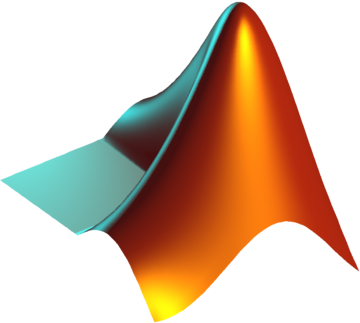
\includegraphics[scale=0.5]{img/MatlabLogo}
	\caption*{Logo de MATLAB}
\end{figure}
\end{frame}

\section {Ventajas}
\begin{frame}{Ventajas de usar \textbf{MATLAB}}{}
	\begin{itemize}
		\item MATLAB nos facilita la manipulación de matrices al trabajar con grandes cantidades de datos.
		\item Posee una gran cantidad de funciones útiles para análisis numéricos.
		\item Nos permite crear interfaces de usuario GUI de una manera fácil y rápida.
		\item Poseé herramientas que nos permiten vincular con otros lenguajes de programación y dispositivos de hardware. 
	\end{itemize}

\end{frame}
\section{Gráficas}
\begin{frame}{Gráficas}{Gráficas bidimensionales}
	\begin{figure}[ht]
		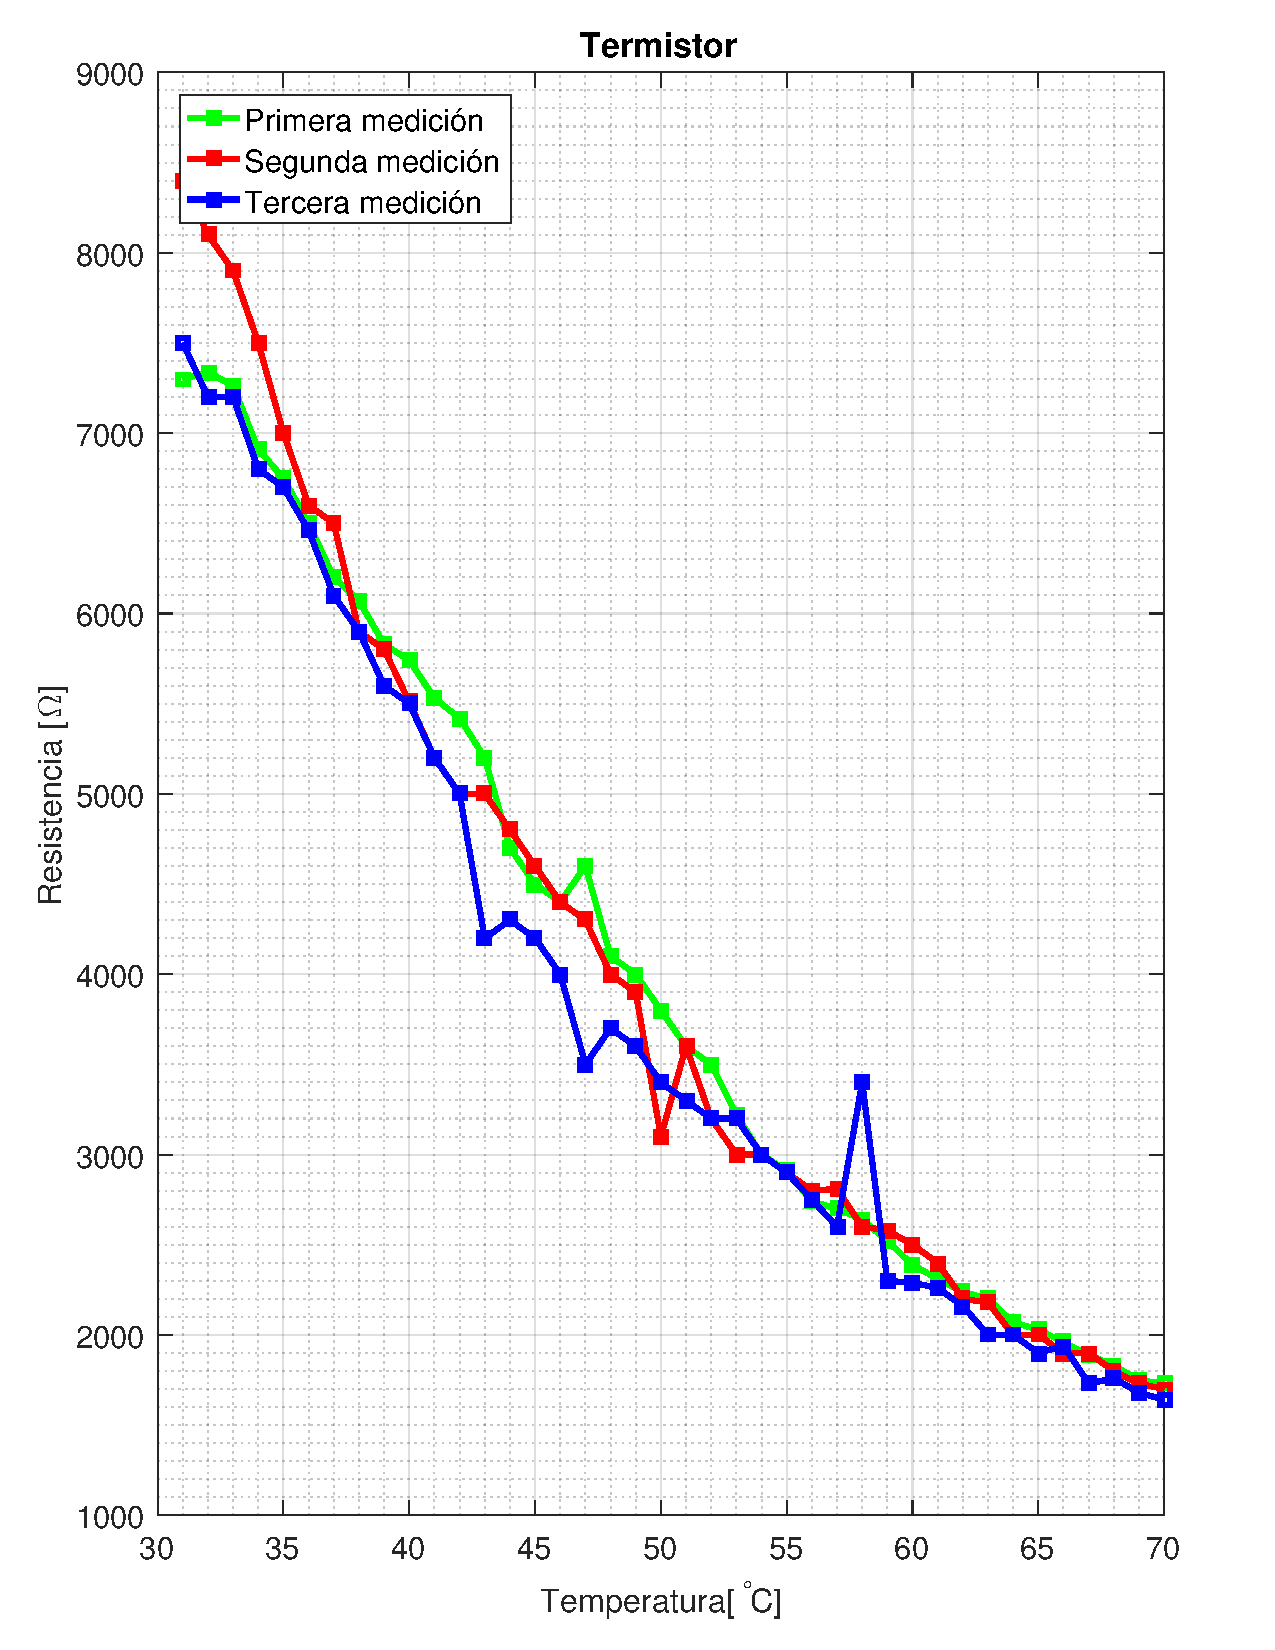
\includegraphics[scale=0.2]{img/termistor}
		\caption*{Gráfica bidimensional}
	\end{figure}

\end{frame}

\begin{frame}{Interpolación}{}
	\begin{figure}[ht]
	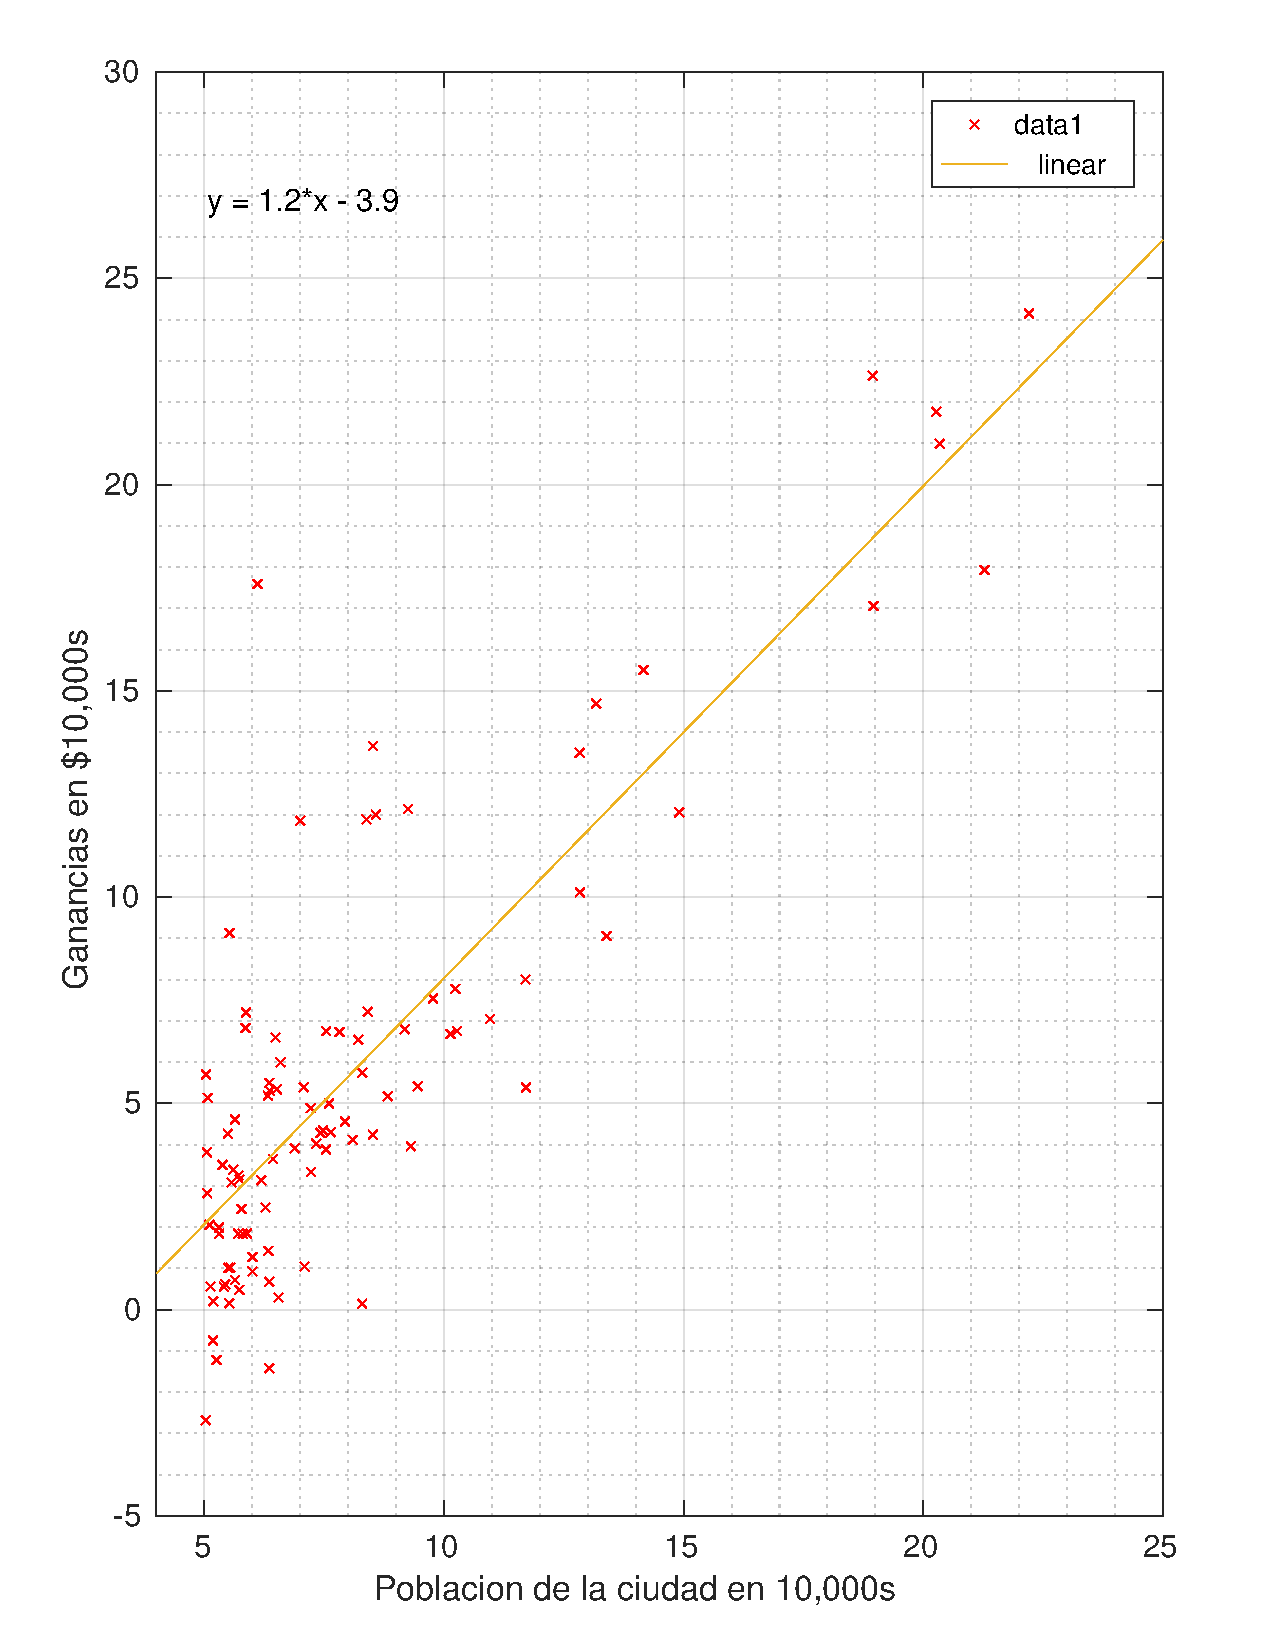
\includegraphics[scale=0.2]{img/regresion}
	\caption*{interpolación}
\end{figure}

\end{frame}

\begin{frame}{Gráficas en 3D}{}
	\begin{figure}[ht]
	\includegraphics[scale=0.2,width=0.5\linewidth]{img/td}
	\caption*{Gráfica tridimensional}
\end{figure}
\end{frame}
\section{Análisis numérico}
\begin{frame}{Cálculo simbólico}{}
\textbf{Límites de funciones}
\[
	fx=\frac{2x^4-12x^3+19x^2-18x+24}{x^3-4x^2-4x+16}
\]
\textbf{Derivadas e integrales}
\[
f(x)=\log\sqrt\frac{1+\sin(x)}{1-\sin(x)}
\]
\end{frame}

\section{Machine Learning}

\begin{frame}{Inteligencia artificial}{Machine Learning}
El machine learning es una rama de la inteligencia artificial que tiene varias definiciones, una de ellas es: ``\textit{Es el campo de estudio que le da a los ordenadores la habilidad de aprender algo sobre lo que no han sido explícitamente programados}"
	\begin{figure}[ht]
	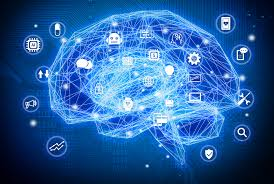
\includegraphics[scale=0.2,width=0.5\linewidth]{img/ML}
\end{figure}
\end{frame}

\begin{frame}{Machine learning}{¿Quién lo usa?}
\begin{figure}[ht]
	\begin{subfigure}{0.5\textwidth}
		
\includegraphics[scale=0.5]{img/netflix}
	\end{subfigure}
	\begin{subfigure}{0.5\textwidth}
		
\includegraphics[scale=0.15]{img/gmail}	
	\end{subfigure}
	\begin{subfigure}{0.5\textwidth}
		
\includegraphics[scale=0.25]{img/facebook}
	\end{subfigure}
\end{figure}
\end{frame}

\end{document}